\documentclass[tikz,border=10pt]{standalone}
\usepackage{tikz}
\usetikzlibrary{shapes.geometric,arrows.meta,positioning,fit,backgrounds,shadows.blur}

\definecolor{greenFill}{HTML}{E8F5E9}
\definecolor{greenStroke}{HTML}{43A047}
\definecolor{memFill}{HTML}{FFF3E0}
\definecolor{memStroke}{HTML}{FFB74D}
\definecolor{coreFill}{HTML}{E1F5FE}
\definecolor{coreStroke}{HTML}{0277BD}
\definecolor{optFill}{HTML}{FCE4EC}
\definecolor{optStroke}{HTML}{E91E63}
\definecolor{procFill}{HTML}{FFF9C4}
\definecolor{procStroke}{HTML}{FBC02D}
\definecolor{textMain}{HTML}{263238}
\definecolor{textMuted}{HTML}{607D8B}

\begin{document}
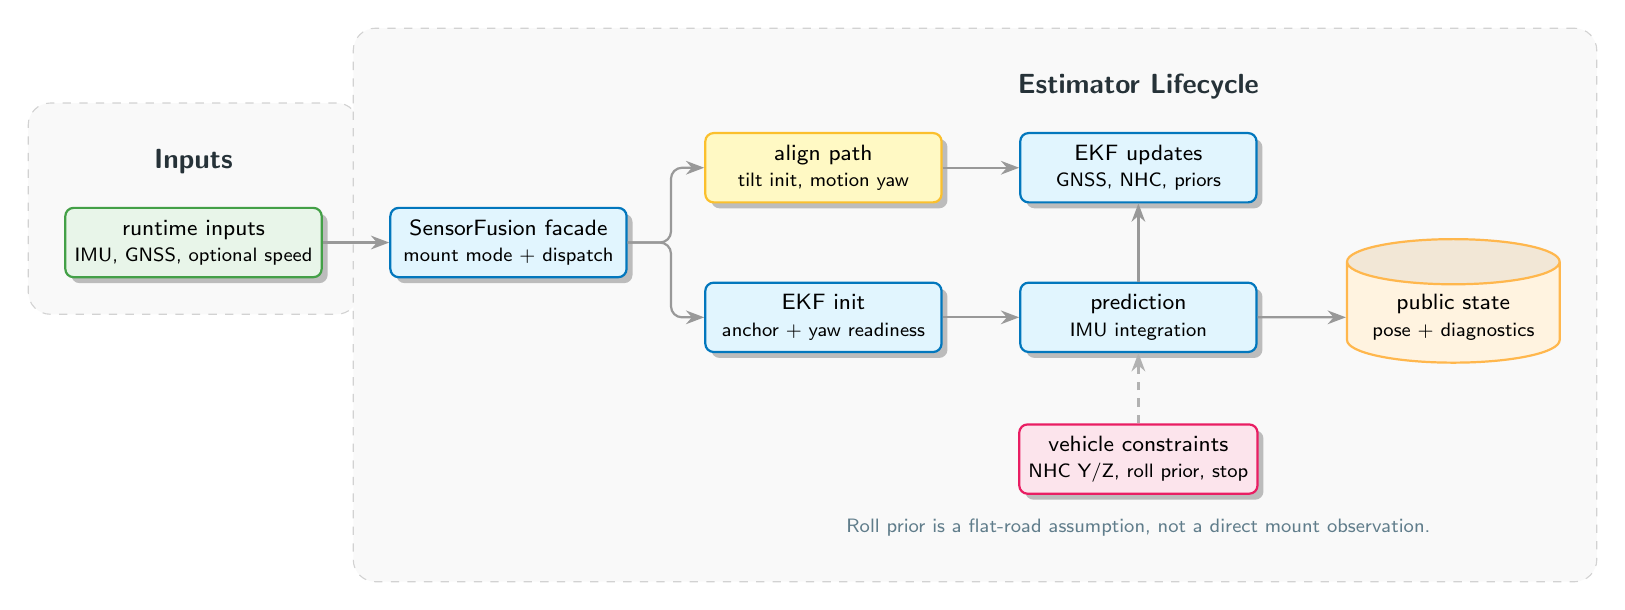
\begin{tikzpicture}[
    node distance=0.7cm and 1.35cm,
    font=\sffamily\footnotesize,
    >=Stealth,
    dataNode/.style={
        rectangle, rounded corners=3pt,
        draw=greenStroke, thick,
        fill=greenFill,
        minimum width=3.0cm, minimum height=0.88cm,
        align=center,
        drop shadow
    },
    opNode/.style={
        rectangle, rounded corners=3pt,
        draw=coreStroke, thick,
        fill=coreFill,
        minimum width=3.0cm, minimum height=0.88cm,
        align=center,
        drop shadow
    },
    procNode/.style={
        rectangle, rounded corners=3pt,
        draw=procStroke, thick,
        fill=procFill,
        minimum width=3.0cm, minimum height=0.88cm,
        align=center,
        drop shadow
    },
    optNode/.style={
        rectangle, rounded corners=3pt,
        draw=optStroke, thick,
        fill=optFill,
        minimum width=3.0cm, minimum height=0.88cm,
        align=center,
        drop shadow
    },
    memNode/.style={
        cylinder, cylinder uses custom fill,
        cylinder body fill=memFill, cylinder end fill=memFill!90!gray,
        shape border rotate=90,
        aspect=0.25,
        draw=memStroke, thick,
        minimum width=2.7cm, minimum height=1.0cm,
        align=center
    },
    group/.style={
        draw=gray!35, dashed, rounded corners=8pt,
        inner sep=13pt, fill=gray!5
    },
    title/.style={font=\sffamily\bfseries, text=textMain, align=center},
    note/.style={font=\sffamily\scriptsize, text=textMuted, align=center},
    flow/.style={->, thick, draw=gray!80, rounded corners=4pt},
    support/.style={->, thick, dashed, draw=gray!60, rounded corners=4pt}
]

% Layout plan: one main lifecycle line, with constraints entering updates from below.
\node[dataNode] (Inputs) at (0, 0.8)
  {runtime inputs\\\scriptsize IMU, GNSS, optional speed};
\node[title, above=0.3cm of Inputs] (InputTitle) {Inputs};

\node[opNode] (Facade) at (4.0, 0.8) {SensorFusion facade\\\scriptsize mount mode + dispatch};
\node[procNode] (Align) at (8.0, 1.75) {align path\\\scriptsize tilt init, motion yaw};
\node[opNode] (Init) at (8.0, -0.15) {EKF init\\\scriptsize anchor + yaw readiness};
\node[opNode] (Updates) at (12.0, 1.75) {EKF updates\\\scriptsize GNSS, NHC, priors};
\node[opNode] (Predict) at (12.0, -0.15) {prediction\\\scriptsize IMU integration};
\node[memNode] (State) at (16.0, -0.15) {public state\\\scriptsize pose + diagnostics};
\node[optNode] (Constraints) at (12.0, -1.95)
  {vehicle constraints\\\scriptsize NHC Y/Z, roll prior, stop};
\node[note, below=0.18cm of Constraints] (ConstraintNote)
  {Roll prior is a flat-road assumption, not a direct mount observation.};
\node[title, above=0.3cm of Updates] (LifecycleTitle) {Estimator Lifecycle};

\begin{scope}[on background layer]
  \node[group, fit=(InputTitle)(Inputs)] {};
  \node[group, fit=(LifecycleTitle)(Facade)(Align)(Init)(Updates)(Predict)(State)(Constraints)(ConstraintNote)] {};
\end{scope}

\draw[flow] (Inputs.east) -- (Facade.west);
\draw[flow] (Facade.east) -- ++(0.55,0) |- (Align.west);
\draw[flow] (Facade.east) -- ++(0.55,0) |- (Init.west);
\draw[flow] (Align.east) -- (Updates.west);
\draw[flow] (Init.east) -- (Predict.west);
\draw[flow] (Predict.north) -- (Updates.south);
\draw[flow] (Predict.east) -- (State.west);
\draw[support] (Constraints.north) -- (Predict.south);

\end{tikzpicture}
\end{document}
